
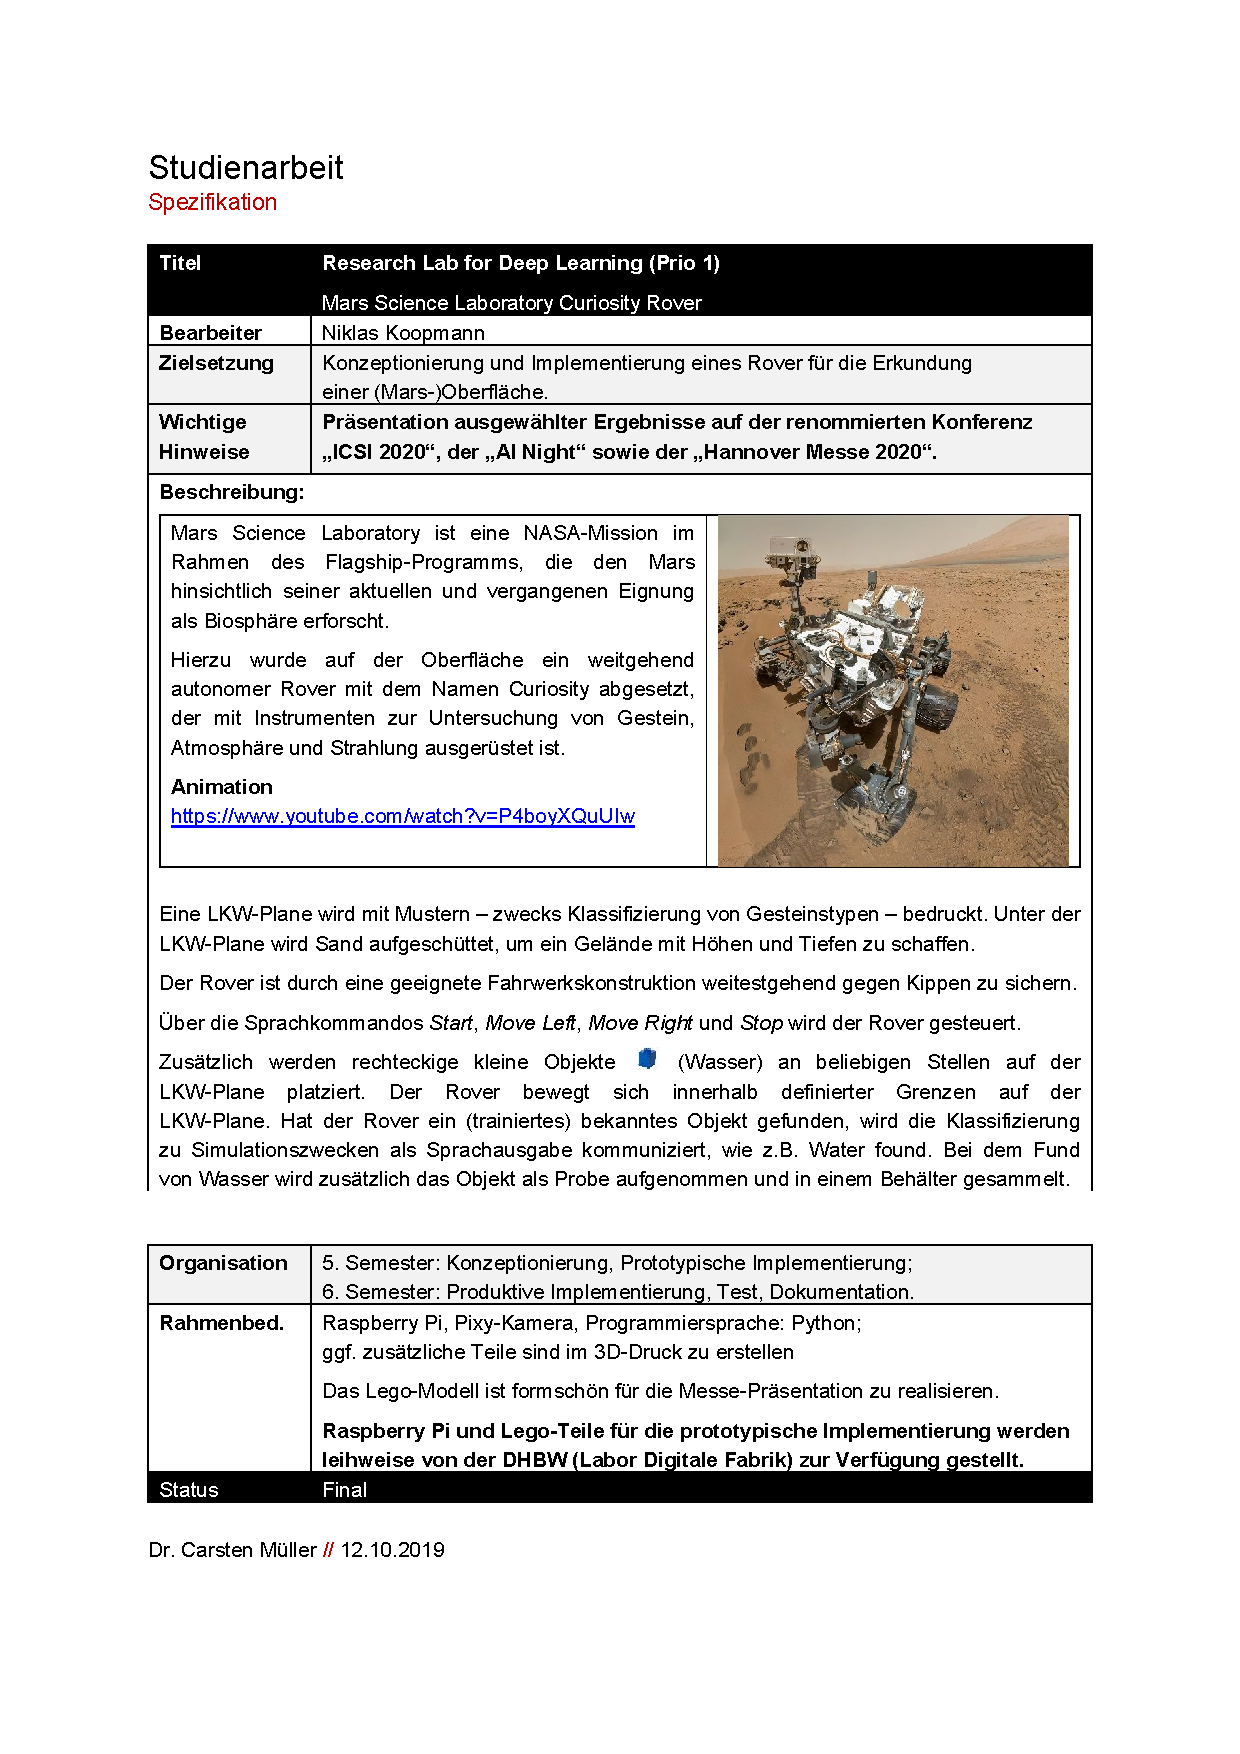
\includepdf[scale=0.8, pages=1, offset=0 -1cm, pagecommand={\chapter{Spezifikation} \label{chp:spezifikation}}]{content/spec.pdf}
\includepdf[scale=0.8, pages=2-, offset=0 -1cm, pagecommand={}]{content/spec.pdf}

\section{Motivation}
\label{sec:motivation}

Am 6. August 2012 landete der Rover \textit{Curiosity} als Teil der Mission \textit{Mars Science Laboratory} der US-amerikanischen Raumfahrtbehörde \acf{nasa} im Gale-Krater auf dem Mars \cite{vasavada2014}.
Seither hat er rund $21{,}93$ Kilometer zurückgelegt (Stand: Sol 2695) \cite{nasa2020} und die Landschaft entlang der Fahrtstrecke auf vielfältige Weise im Hinblick auf ihre frühere und aktuelle Eignung als Lebensraum für Organismen untersucht.
Ein wichtiger Aspekt für den Nachweis der Existenz von Lebewesen ist das Vorhandensein flüssigen Wassers \cite{nasa2013}, dessen Rückstände der Rover mithilfe eines aktiven Neutronenspektrometers in Mineralien nachzuweisen versucht. \cite{vasavada2014}

Um weite Strecken im schroffen, unebenen Gelände der Marsoberfläche zurücklegen zu können, ist \textit{Curiosity} mit einem komplexen, sechsrädrigen Antriebs- und Federungssystem ausgestattet.
Das Fahrwerk ist nach dem Rocker-Bogie-System der \acs{nasa} aufgebaut, um Hindernisse bis zu einer Höhe des Raddurchmessers von $0{,}5\ m$ überwinden zu können \cite{arvidson2013}.
Eine solche Aufhängung ermöglicht dem Rover eine hohe Geländegängigkeit ohne den Einsatz von Achsen und erlaubt der Verbindung der hinteren Räder beider Seiten eine freie Drehung um den Verbindungspunkt zur Hauptstrebe, an der auch das jeweilige Vorderrad montiert ist \cite{bickler1998}. 

% TODO Weitere Ausführungen

Dieses Projekt (Mars Science Laboratory Curiosity Rover) wird im Rahmen des Research Lab for Deep Learning der Dualen Hochschule Baden-Württemberg (\acsu{dhbw}) zeitgleich mit der Erforschung schwarmbasierter Logistikabläufe durchgeführt.
Langfristig soll das Ergebnis unter anderem zum Zwecke einer schwarmbasierten Erkundung marsähnlicher Landschaften weiterentwickelt werden können.

\section{Aufgabenstellung}
\label{sec:aufgabe}

Ziel dieser Arbeit ist die \glqq Konzeptionierung und Implementierung eines Rover für die Erkundung einer (Mars-)Oberfläche\grqq\ \cite{mueller2019}.
Die Suche nach Wasser wird dabei ebenfalls abgebildet und soll mithilfe der visuellen Erkennung blauer LEGO-Steine simuliert werden.
Zusätzlich ist das Antriebskonzept des \textit{Curiosity}-Rovers originalgetreu nachzubilden: Es sollen sechs angetriebene Räder installiert sein, von denen vier gelenkt werden.
Eine grundlegende mechanische Federung soll die Geländetauglichkeit steigern.

In einzelnen Punkten ist nachträglich einvernehmlich von der Spezifikation abgewichen worden:
Der Rover muss keine Wasserobjekte aufsammeln können.
Wenn ein Wasserobjekt erkannt wird, soll dies lediglich über die Sprachausgabe verkündet werden.
Der Fokus der Entwicklung ist von der Geländetauglichkeit hin zur Stabilität und Formschönheit gerückt worden.
Das klassische Rocker-Bogie-Fahrwerk wird im Sinne der Originaltreue in leicht abgewandelter Form verbaut (siehe dazu Abschnitt \ref{sec:seitenansicht}).

% TODO REMOVE LITERATURE TESTS
Literatur-Test:
\cite{yamanoor2017}
\cite{horan2013}
\cite{donat2018}
\cite{halfacree2019}
\cite{mcmanus2017}
\cite{cox2014}